\documentclass{beamer} 

\usepackage[utf8]{inputenc}
\usepackage[T1]{fontenc}
\usepackage{graphicx}
\usepackage[serbian]{babel}
\usepackage{multicol}
\usepackage{tikz}
\usetikzlibrary{shapes.geometric, arrows}


\usetheme{default}
\begin{document}


% TikZ blok dijagram stilovi
\tikzstyle{block} = [rectangle, rounded corners, minimum width=3cm, minimum height=1cm, text centered, draw=black, fill=blue!30]
\tikzstyle{arrow} = [thick,->,>=stealth]

\title{Evaluation and analysis of graph vertex embeddings based on information-oriented random walks in distributed environment with community-aware vertex partitioning}
\author{Stefan Nožinić \\
Departman za matematiku i informatiku \\
Prirodno-matematički fakultet \\
Univerzitet u Novom Sadu \\
}
\date{23. novembar 2025.}

\frame{
\titlepage
}

\section{Uvod i motivacija}
\begin{frame}{Uvod}
    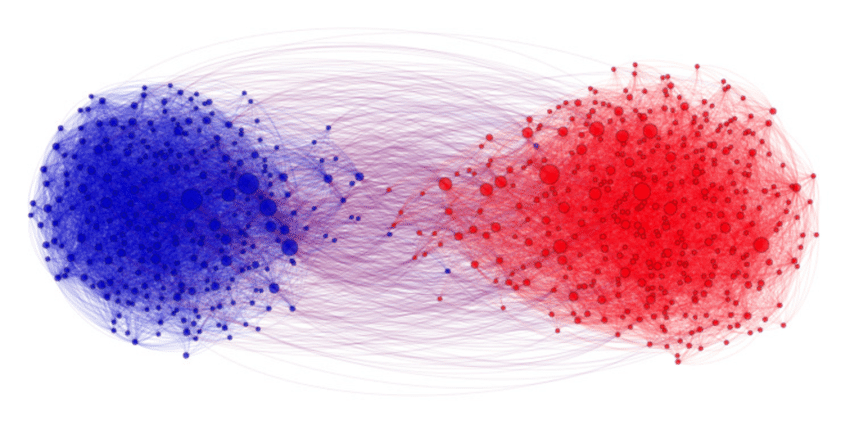
\includegraphics[width=\textwidth]{png/uvod.png}
    % add footnote
    \begin{tiny}
        Izvor: Interian, Ruben i Ribeiro, Celso. (2018). An empirical investigation of network polarization. Applied Mathematics and Computation. 339. 651-662. 10.1016/j.amc.2018.07.066.
    \end{tiny}
\end{frame}

\begin{frame}
	\frametitle{Ugrađivanje (embedovanje) čvorova}
	Neka je $ G = (V, E) $ graf, tada je ugrađivanje (embedovanje) funkcija 

	$$ U : V \to \mathbb{R}^n $$ 

	koja preslikava čvorove grafa u n-dimenzionalni euklidski prostor tako da čvorovi koji su dosta međusobno povezani budu blizu po euklidskom rastojanju
	

\end{frame}

\begin{frame}{node2vec algoritam}
	\centering
    \begin{tikzpicture}[node distance=2cm]

    % Blokovi
    \node (walks) [block] {Slučajne šetnje po čvorovima grafa};
    \node (embedding) [block, below of=walks] {Ugrađivanje (Embedding)};

    % Strelice
    \draw [arrow] (walks) -- (embedding);

    \end{tikzpicture}
\end{frame}

\begin{frame}
    \frametitle{DistGER}

$$ 
\alpha(u,v) =
\frac{1}{\deg(u) - C_m(u,v)}
\cdot
\max\left(
\frac{\deg(u)}{\deg(v)},
\frac{\deg(v)}{\deg(u)}
\right)
$$


$$
Z(x) = \frac{e^{x} - e^{-x}}{e^{x} + e^{-x}} = \tanh(x)
$$
    
\end{frame}

\begin{frame}
    \frametitle{Određivanje dužine šetnje}
$$
r(H,L) =
\frac{
\sum_{i=1}^n (H_i - \bar{H})(L_i - \bar{L})
}{
\sqrt{\sum_{i=1}^n (H_i - \bar{H})^2}
\sqrt{\sum_{i=1}^n (L_i - \bar{L})^2}
}
$$
    
\end{frame}

\begin{frame}{Ciljevi istraživanja}
    \begin{itemize}
        \item Implementacija paralelne verzije node2vec algoritma i DistGER algoritma u distribuiranom okruženju
        \item Implementacija metoda particionisanja grafa koje su svesne zajednica
        \item Analiza gubitka strukturnih informacija usled particionisanja
        \item Evaluacija performansi na velikim realnim mrežama
        \item Poređenje kvaliteta dobijenog ugrađivanja sa serijskom verzijom
    \end{itemize}
\end{frame}


\section{Arhitektura}
\begin{frame}{Arhitektura}
    \centering
    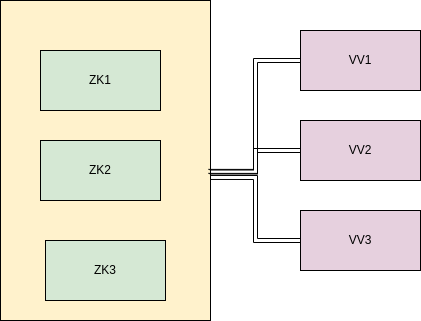
\includegraphics[height=0.8\textheight]{./png/Arhitektura i infrastruktura.drawio.png}
\end{frame}

\begin{frame}{Način rada - master i radni čvorovi}
    \begin{columns}
        \begin{column}{0.5\textwidth}
            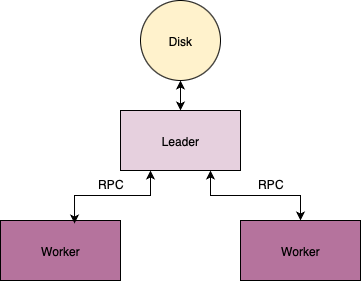
\includegraphics[height=0.5\textheight]{./png/Classic mode.drawio.png}
    \end{column}
    \begin{column}{0.5\textwidth}
        \begin{itemize}
            \item Master čvor:
            \begin{itemize}
                \item Učitava graf iz baze podataka
                \item Particioniše graf
                \item Raspoređuje particije po radnim čvorovima
                \item Prikuplja rezultate od radnih čvorova
                \item Spaja rezultate u konačno ugrađivanje
            \end{itemize}
            \item Radni čvorovi:
            \begin{itemize}
                \item Učitavaju particiju grafa iz baze podataka
                \item Izvršavaju node2vec algoritam na učitanom delu grafa
                \item Šalju rezultate nazad master čvoru
            \end{itemize}
        \end{itemize}
    \end{column}
    \end{columns}
\end{frame}

\begin{frame}{Način rada - Deljeni resursi}
    \begin{columns}
        \begin{column}{0.5\textwidth}
            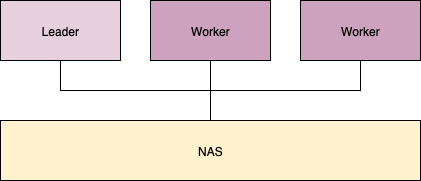
\includegraphics[width=0.5\textheight]{./png/NAS mode.drawio.png}
        \end{column}
        \begin{column}{0.5\textwidth}
            \begin{itemize}
                \item Izabere se jedan glavni čvor koji radi koordinaciju zadataka.
                \item Koordinator prosleđuje reference ka particijama
                \item Svi procesi imaju deljeno skladište za podatke
                \item Značajno pogodnije da se koristi sa integracijom sa SLURM-om.
            \end{itemize}
        \end{column}
    \end{columns}
\end{frame}

\section{Blokovski prikaz algoritma}
\begin{frame}{Blokovski prikaz algoritma}
    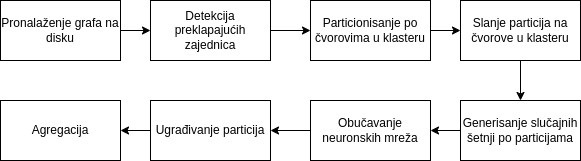
\includegraphics[width=\textwidth]{./png/Blokovski prikaz algoritma.drawio.png}
\end{frame}

\begin{frame}{Particionisanje po čvorovima u klasteru}
    \begin{itemize}
        \item Nakon detekcije zajednica, potrebno je rasporediti zajednice po čvorovima u klasteru
        \item U ovom radu, korišćen je bin packing algoritam
        \item Algoritam raspoređuje zajednice po čvorovima, tako da čvorovi u klasteru budu što sličniji po svom opterećenju
        \item Opterećenje čvora K, kom su raspoređene zajednice $ S_K $, je $ \sum_{s \in S_K} |s| $
        \item Težine se zatim sortiraju u opadajućem redosledu, počevši od najveće.
        \item Inicijalno, maksimalna veličina (kapacitet) particije je prosečna veličina zajednice 
    \end{itemize}
\end{frame}

\begin{frame}
    \frametitle{Particionisanje - LPA algoritam}
    \begin{itemize}
        \item Algoritam zasnovan na širenju oznaka (Label Propagation Algorithm - LPA)
        \item Inicijalno, svaki čvor ima jedinstvenu oznaku
        \item U svakoj iteraciji, svaki čvor ažurira svoju oznaku na onu koja je najčešća među njegovim susedima
        \item Proces se ponavlja dok se oznake ne stabilizuju
        \item Nakon što su zajednice detektovane, koristi se isti bin packing algoritam za raspoređivanje zajednica po čvorovima u klasteru
    \end{itemize}
\end{frame}

\begin{frame}
    \frametitle{Particionisanje po čvorovima u klasteru}
    \begin{itemize}
        \item Algoritam dodeljuje particije zajednicama, počevši od najveće zajednice. Uvek se dodeljuje particija koja je najmanje opterećena
        \item Ukoliko ne postoji particija koja ima potreban kapacitet, kapacitet particija se povećava za prosečnu veličinu zajednice koja još nije dodeljena particiji. 
        \item Ovaj proces se ponavlja dok sve zajednice ne budu raspoređene.
    \end{itemize}
\end{frame}


\section{Gubici strukturnih informacija}
\begin{frame}{Mera gubitka strukturnih informacija}
    \begin{columns}
		\begin{column}{0.5\textwidth}
            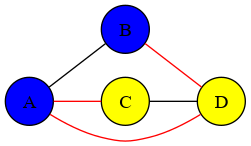
\includegraphics[width=\textwidth]{dot/graf.png}
		\end{column}
		\begin{column}{0.5\textwidth}
            Neka je $ E_p $ skup svih grana koje sadrže čvorove takve da su oba čvora u particiji $ p $  i neka je $ P $ skup svih particija za graf $ G = (V, E) $
            
            Tada je mera gubitka strukturnih informacija $ L $ definisana kao
            
            $$ L = 1-\frac{\sum_{p \in P} |E_p|}{|E|} $$
            
            , gde je $ |E_p| $ broj grana koje sadrže čvorove iz particije $ p $, a $ |E| $ ukupan broj grana u grafu $ G $.
		\end{column}
	\end{columns}
\end{frame}

\section{Korišćeni skupovi podataka}
\begin{frame}{Skupovi podataka}
    \begin{itemize}
        \item CITESEER
        \item AstroPh
        \item Cit-HepPh
    \end{itemize}
\end{frame}


\begin{frame}{Karakteristike mreža korišćenih u eksperimentima}
\begin{table}[h!]
\centering
\begin{tabular}{lccc}
\hline
\textbf{Mreža} & \textbf{\# čvorova} & \textbf{\# grana} & \textbf{Koef. klasterizacije} \\
\hline
CITESEER   & 3264   & 4532    & 0.14 \\
AstroPh    & 18772  & 198110  & 0.63 \\
Cit-HepPh  & 34546  & 420921  & 0.28 \\
\hline
\end{tabular}
\caption{Karakteristike mreža korišćenih u eksperimentima.}
\end{table}
\end{frame}

\begin{frame}{F1 skorovi za Node2Vec sa Label Propagation (4 particije)}
\begin{table}[h!]
\centering
\begin{tabular}{lc}
\hline
\textbf{Mreža} & \textbf{F$_1$ na 4 čvora} \\
\hline
CITESEER   & 44.34\% \\
AstroPh    & 19.48\% \\
Cit-HepPh  & 4.8\% \\
\hline
\end{tabular}
\caption{F1 skorovi za distribuirani Node2Vec sa label propagation algoritmom (4 particije).}
\end{table}
\end{frame}


\begin{frame}{F1 skorovi za DistGER sa Label Propagation}
\begin{table}[h!]
\centering
\begin{tabular}{lccc}
\hline
\textbf{Mreža} & \textbf{1 čvor} & \textbf{2 čvora} & \textbf{4 čvora} \\
\hline
CITESEER   & 22.14\% & 43.83\% & 60.66\% \\
AstroPh    & 5.53\%  & 8.05\%  & 29.77\% \\
Cit-HepPh  & 2.68\%  & 4.04\%  & 4.39\% \\
\hline
\end{tabular}
\caption{F1 skorovi za DistGER sa label propagation particionisanjem (1, 2 i 4 čvora).}
\end{table}
\end{frame}

\begin{frame}{Balans i edge cut za Label Propagation (4 particije)}
\begin{table}[h!]
\centering
\begin{tabular}{lcc}
\hline
\textbf{Mreža} & \textbf{Balans (LPA)} & \textbf{Edge cut (LPA)} \\
\hline
CITESEER   & 0.000612 & 22\% \\
AstroPh    & 0.824    & 8.4\% \\
Cit-HepPh  & 0.00005  & 20.6\% \\
\hline
\end{tabular}
\caption{Balans i edge cut za label propagation na realnim mrežama (4 particije).}
\end{table}
\end{frame}


\begin{frame}{Zaključak}
Distribuirano ugrađivanje čvorova grafa sa particionisanjem zasnovanim na zajednicama pokazalo se kao efikasan način za generisanje visokokvalitetnih reprezentacija, uz očuvanje strukture zajednica u grafu.

\vspace{0.3cm}

Algoritam \textbf{label propagation} pokazao se kao efikasan metod za particionisanje grafova, gde je postigao dobro balansirane particije i mali broj grana čiji su krajevi u različitim particijama.

\vspace{0.3cm}

Metod \textbf{DistGER} ostvario je bolje performanse od \textbf{Node2Vec} prema F1 meri rekonstrukcije, što ukazuje na to da maksimizacija informacionog dobitka tokom generisanja slučajnih šetnji dovodi do boljih ugrađivanja.
\end{frame}




\begin{frame}
	\begin{center}
		\Huge Hvala na pažnji!
	\end{center}
\end{frame}


\end{document}
